\documentclass[a4paper, 12pt]{article}
\usepackage[utf8]{inputenc}
\usepackage{comment}
\usepackage[spanish]{babel}
\usepackage[margin=1.2in]{geometry}
\usepackage{hyperref}
\usepackage{adjustbox}
\hypersetup{
    colorlinks=true,
    linkcolor=black,
    filecolor=magenta,
    urlcolor=cyan,
}
\usepackage{caption}
\geometry{top = 1in}
\setlength{\textfloatsep}{1\baselineskip plus 0.2\baselineskip minus 0.5\baselineskip}
\setlength{\parindent}{2em}
\renewcommand\textfraction{.1}
\usepackage{float}

\title{Competencia de Machine Learning \\ Trabajo práctico 2 - Organización de Datos}
\author{Grupo: \textit{Back to the Data}}
\date{24/06/19}

\usepackage{natbib}
\usepackage{graphicx}
\newcommand\tab[1][1cm]{\hspace*{#1}}
\usepackage{placeins}

\begin{document}
\begin{figure}
    \centering
    \makebox[\textwidth]{
\includegraphics[width=250pt]{logofiuba.jpg}}
\end{figure}
\maketitle

\FloatBarrier
\begin{center}
	\begin{adjustbox}{width=1\textwidth}
        \begin{tabular}{ |c|c|c| }
          \hline
          Nombre & Padrón & Mail \\
          \hline\hline
          Álvarez, Federico & 99266 & fede.alvarez1997@gmail.com \\
          \hline
          La Torre, Gabriel & 87796 & latorregab@gmail.com \\
          \hline
          Medrano, Lucas Nicolás & 99247 & lucasmedrano97@gmail.com \\
          \hline
          Piro Martino, Ariel & 99469 & ariel.piro@hotmail.com \\
          \hline
       	 \end{tabular}
       \end{adjustbox}
\end{center}
\FloatBarrier

\newpage

\tableofcontents
\newpage

\section{Introducción}
El trabajo consiste en participar en una competencia de machine learning. 

La empresa Jampp provee información sobre subastas, clicks, instalaciones y eventos en dispositivos móviles, y el objetivo es estimar, para un conjunto dado de dispositivos, el tiempo que tardará cada uno en aparecer nuevamente en una
subasta o que se instale en él una nueva aplicación.

Llamaremos $St(d)$ al tiempo que transcurre hasta que un dispositivo d aparezca nuevamente en una subasta, y $Sc(d)$ al tiempo que transcurre hasta que el dispositivo d convierta (instale una nueva aplicación)


Los datasets contienen información del 18/06 al 26/06 inclusive.
Para entrenar los algoritmos, se dividió la información en 7 ventanas (ambos extremos de todas las ventanas son incluyentes):

\begin{itemize}
    \item Ventana 1) 18/06 - 20/06 \item Ventana 2) 19/06 - 21/06
    \item Ventana 3) 20/06 - 22/06 \item Ventana 4) 21/06 - 23/06
    \item Ventana 5) 22/06 - 24/06 \item Ventana 6) 23/06 - 25/06
    \item Ventana 7) 24/06 - 26/06
\end{itemize}

Los algoritmos usan como set de entrenamiento los tres días de una ventana, y validan con los siguientes tres días.

La realización se dividió en 4 procesos que se describen en las siguientes secciones.
Primero, el pre-procesamiento - análisis y filtrado - de los datos. Luego una primer prueba con algún algoritmo simple de implementar. A continuación se probaron distintos algoritmos solamente con las columnas que quedaron luego del pre-procesamiento, con búsqueda de parámetros e hipeparámetros. Por último se hizo una etapa de feature engineering buscando nuevos features para volver a correr los algoritmos que se habían implementado en la etapa anterior y comparar resultados.

Todos los algoritmos y procesos se pueden encontrar en el siguiente repositorio de GitHub: \href{https://github.com/shizus/7506-1c2019}{https://github.com/shizus/7506-1c2019}.

\newpage
\section{Pre-procesamiento}
Lo primero que se hizo en el trabajo es un análisis de los datos recibidos. El objetivo era borrar features (o columnas) que se supiera de antemano no iban a influir en el aprendizaje de los algoritmos, como por ejemplo aquellas que tuvieran únicamente valores nulos, un solo valor para todas las filas o un valor diferente para cada fila, y decidir que hacer con las demás columnas (aquellas que tuvieran solo algunos valores nulos, por ejemplo).

A continuación se explicitan las decisiones tomadas para las columnas que presentaron conflictos (entendiendo como conflictos los mencionados en el párrafo anterior)

En las siguientes secciones se indican en una tabla las columnas conflictivas, qué se decidió hacer con cada una y el motivo. Las columnas que no aparecen mencionadas no necesitaron ninguna acción por parte del grupo.

\subsection{clicks.csv}

\FloatBarrier
\begin{center}
        \begin{tabular}{ |c|c|c| }
          \hline
          Columna & Acción & Motivo \\
          \hline\hline
          auction\_id & Eliminada & Todos valores nulos \\
          \hline
          country\_code & Eliminada & Hay un solo país \\
          \hline
          trans\_id & Eliminada & Todos valores distintos. \\
          \hline
          agent\_device & Eliminada & Casi ningún valor no nulo. \\
          \hline
          brand & Eliminada & Casi ningún valor no nulo \\
          \hline
          carrier\_id & Rellenada & Tiene muy pocos valores nulos \\
          \hline
          os\_major & Rellenada & Tiene muy pocos valores nulos \\
          \hline
          os\_minor & Rellenada & Tiene muy pocos valores nulos \\
          \hline
          timeToClick & Rellenada & Tiene muy pocos valores nulos \\
          \hline
          touchX & Rellenada & Tiene muy pocos valores nulos \\
          \hline
          touchY & Rellenada & Tiene muy pocos valores nulos \\
          \hline
        \end{tabular}
\end{center}
\FloatBarrier
Los valores nulos de la columna timeToClick, touchsX y touchsY se rellenaron con el promedio de cada columna.

\subsection{installs.csv}
\FloatBarrier
\begin{center}
	\begin{adjustbox}{width=1\textwidth}
        \begin{tabular}{ |c|c|c| }
          \hline
          Columna & Acción & Motivo \\
          \hline\hline
          trans\_id & Eliminada & 98\% de los valores nulos \\
          \hline
          device\_countrycode & Eliminada & Hay un solo país \\
          \hline
          click\_hash & Eliminada & 99\% de los valores nulos \\
          \hline
          event\_uuid & Eliminada & Casi 80\% de los valores nulos \\
          \hline
          kind & Eliminada & Casi 80\% de los valores nulos \\
          \hline
          wifi & Eliminada & Casi 50\% de los valores nulos \\
          \hline
          device\_brand & Eliminada & 42\% de los valores nulos \\
          \hline
          user\_agent & Eliminada & 30\% de los valores nulos \\
          \hline
          session\_user\_agent & Filas nulas eliminadas & 3\% de los valores nulos \\
          \hline
          device\_model y device\_language & Filas nulas eliminadas & Juntas son el 5\% de los valores del dataframe, y son nulos \\
          \hline
        \end{tabular}
	\end{adjustbox}
\end{center}
\FloatBarrier

\subsection{auctions.csv}
    El dataset de auctions no tenía valores nulos ni columnas conflictivas, por lo que se usó como estaba.

\subsection{events.csv}
\FloatBarrier
\begin{center}
        \begin{tabular}{ |c|c|c| }
          \hline
          Columna & Acción & Motivo \\
          \hline\hline
          trans\_id & Eliminada & casi 100\% de los valores nulos (99,995\%) \\
          \hline
          device\_countrycode & Eliminada & Hay un solo país \\
          \hline
          event\_uuid & Eliminada & Todos los valores distintos \\
          \hline
          device\_os\_version & Eliminada & 70\% de los valores nulos \\
          \hline
          device\_brand & Eliminada & Casi 70\% de los valores nulos \\
          \hline
          device\_city & Eliminada & Casi 80\% de los valores nulos \\
          \hline
          user\_agent & Eliminada & 60\% de los valores nulos \\
          \hline
          carrier & Eliminada & 76\% de los valores nulos \\
          \hline
          connection\_type & Eliminada & Casi 80\% de los valores nulos \\
          \hline
          device\_language & Eliminada & Casi 30\% de los valores nulos \\
          \hline
          session\_ user\_ agent & Filas nulas eliminadas & 0,5\% de los valores nulos \\
          \hline
          kind & Filas nulas eliminadas & 0,5\% de los valores nulos \\
          \hline
          device\_model & Eliminada & casi 30\% de los valores nulos \\
          \hline
        \end{tabular}
\end{center}
\FloatBarrier

\section{Feature engineering}

Para obtener mejores predicciones hubo que modificar las columnas de los sets de entrenamiento.

\subsection{$Sc$}
Para las predicciones del $Sc$ se utilizó como base el archivo \texttt{installs.csv}, que cuenta con información de las instalaciones realizadas por usuarios entre las fechas del 18/04/19 y el 26/04/19. En el mismo figuran el id del dispositivo (ref\_hash), la fecha de instalación, la aplicación, información del dispositivo (ip, modelo, idioma de entrada) y si fue atribuido o no a Jampp. 

Sin embargo, la información presentada de aquella manera no resultaba de utilidad ya que se centraba en la instalación y no en información de los dispositivos. Es por esto que se procedió a modificar el dataframe, agregando las siguientes columnas.

\subsubsection*{total\_apps}
Se calculó para cada dispositivo la cantidad de apps instaladas en el periodo dado, lo cual nos permite observar si el usuario ha realizado instalaciones en el pasado. Este feature va en conjunto con el siguiente y han arrojado buenos resultados para las predicciones.

\subsubsection*{most\_freq\_app}
Este feature indica cúal es la aplicación más instalada para cada dispositivo. Para ello lo que se hizo fue calcular la moda entre las apps instaladas por cada dispositivo, lo cual consumió mucho tiempo ya que esta operación es bastante lenta. 
Afortunadamente este feature resultó de los más importantes a la hora de realizar las predicciones, ya que se ubica en las primeras posiciones en \textit{feature importance} para los diferentes algoritmos.

\subsubsection*{\%implicit y \%attributed}
El dataframe original contaba con dos columnas de tipo booleano que indicaban si la instalación fue atribuia a Jampp y si fue observada por la data orgánica o no. Esta información, si bien resulta útil para la empresa, no podía ser utilizada para las predicciones ya que el archivo \texttt{target\_}\texttt{competencia\_}\texttt{ids.csv} solo contenía ids de dispositivos. Es por esto que lo que se hizo fue calcular el porcentaje de instalaciones implícitas y atribuidas para cada dispositivo, para así contar con información acerca del dispositivo y no de la instalación.

\subsubsection*{most\_freq\_lang, model e ip}
De manera similar al feature sobre las apps, se calculó la moda entre los device\_language, device\_model e ip\_address de cada instalación para cada dispositivo. Esto se hizo para transformar la información original sobre instalaciones en información sobre los dispositivos que fuera útil para predecir. 

Cabe destacar que estos features resultaron de mucha utilidad y rankearon bien en feature importance para distintos algortimos.

Además de la información provista por el dataframe de instalaciones, también se buscó agregarle a éste información sobre los dataframes de clicks y eventos. Sin embargo, esto no fue siempre posible.
Por ejemplo, la información sobre los clicks era muy escasa (el dataframe de clicks tenía aproximadamente el 13\% de la cantidad de filas que tenía el de installs), y los dispositivos que figuraban en ambos eran tan solo 23. Es por esto que se decidió no tener en cuenta los clicks a la hora de agregar features.

En el caso de los eventos, se extrajo la siguiente información detallada en los siguientes features.

\subsubsection*{events\_\%wifi}
Para este feature se extrajo del dataframe de eventos el porcentaje de eventos que cada dispositivo realizó vía wifi. Cabe destacar que como se trata de otro dataframe distinto, hubo algunos dispositivos para los que esta información no estaba, en ese caso se decidió rellenar con 0. Este feature no resultó de mucha utilidad y se lo eliminó posteriormente.

\subsubsection*{event\_apps}
De manera análoga a total\_apps, se calculó la cantidad de aplicaciones para las cuales se registró un evento del dispositivo en cuestión en el periodo dado. Resultó ser de los más importantes a la hora de predecir.

\subsubsection*{distinct\_events y total\_events}
Representando la cantidad de eventos distintos y la cantidad total de eventos generados, estos features no resultaron de gran utilidad, rankeando entre los últimos en importancia, por lo que fueron removidos posteriormente para así mejorar la performance de los algoritmos en cuanto al tiempo se refiere.



Una herramienta muy útil para este proceso fue el mencionado gráfico de importancia de features para los algoritmos. Esto permitía ir verificando a qué darle mayor valor, sobre todo a la hora de ver qué algoritmos promediar, o qué algoritmos usar como columnas para entrenar otros algoritmos.

Por ejemplo, la siguientes imágenes representan la importancia de los diferentes features para los diferentes algoritmos y ensambles utilizados.


\begin{figure}[H]
    \centering
    \makebox[\textwidth]{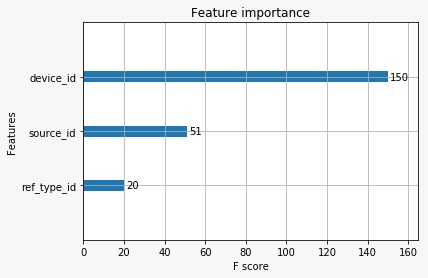
\includegraphics[width=350pt]{xgbst.jpeg}}
    \caption{Feature importance para XGBoost sobre $St$}
\end{figure}

\begin{figure}[H]
    \centering
    \makebox[\textwidth]{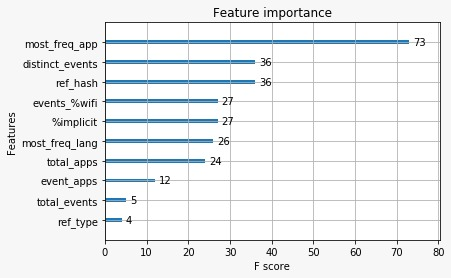
\includegraphics[width=350pt]{xgbsc.jpeg}}
    \caption{Feature importance para XGBoost sobre $Sc$}
\end{figure}

\begin{figure}[H]
    \centering
    \makebox[\textwidth]{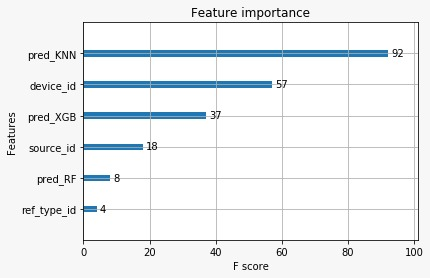
\includegraphics[width=350pt]{xgbknnrfst.jpeg}}
    \caption{Feature importance para el stacking de XGBoost con KNN y Random Forests sobre $St$}
\end{figure}

\begin{figure}[H]
    \centering
    \makebox[\textwidth]{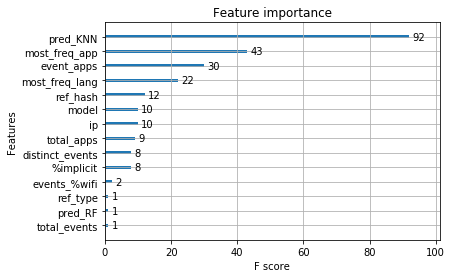
\includegraphics[width=350pt]{featureimportance.png}}
    \caption{Feature importance para el stacking de XGBoost con KNN y Random Forests sobre $Sc$}
\end{figure}

\begin{figure}[H]
    \centering
    \makebox[\textwidth]{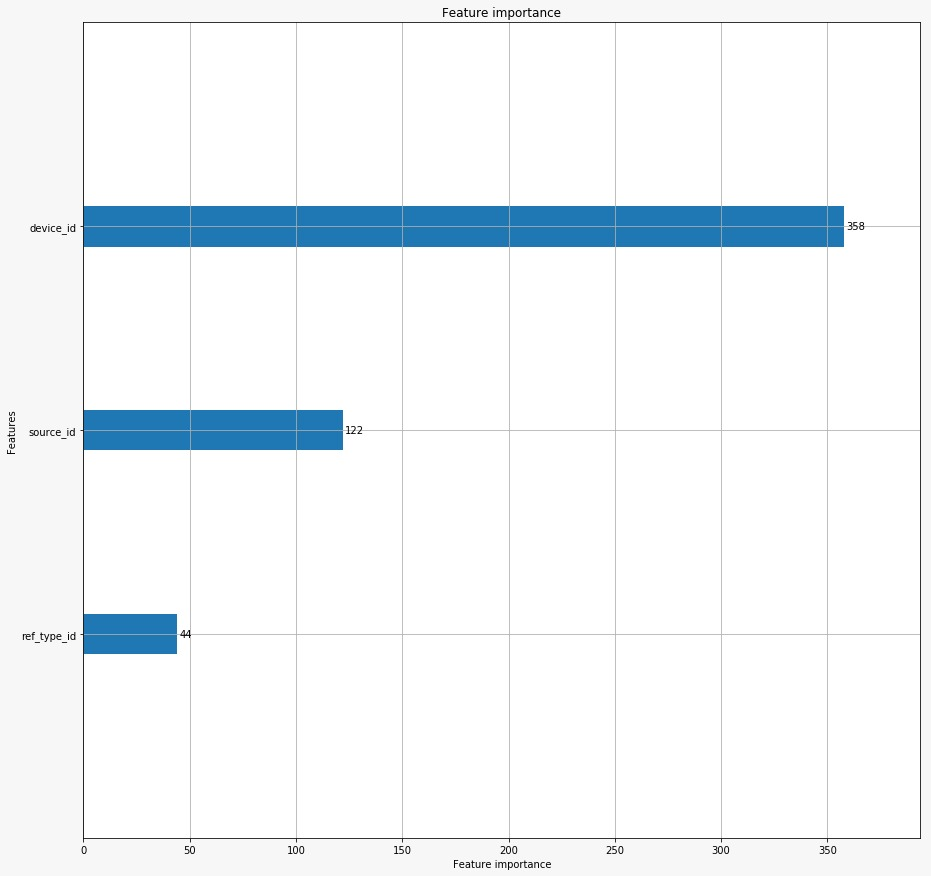
\includegraphics[width=250pt]{lgbmst.jpeg}}
    \caption{Feature importance para LGBM sobre $St$}
\end{figure}

\begin{figure}[H]
    \centering
    \makebox[\textwidth]{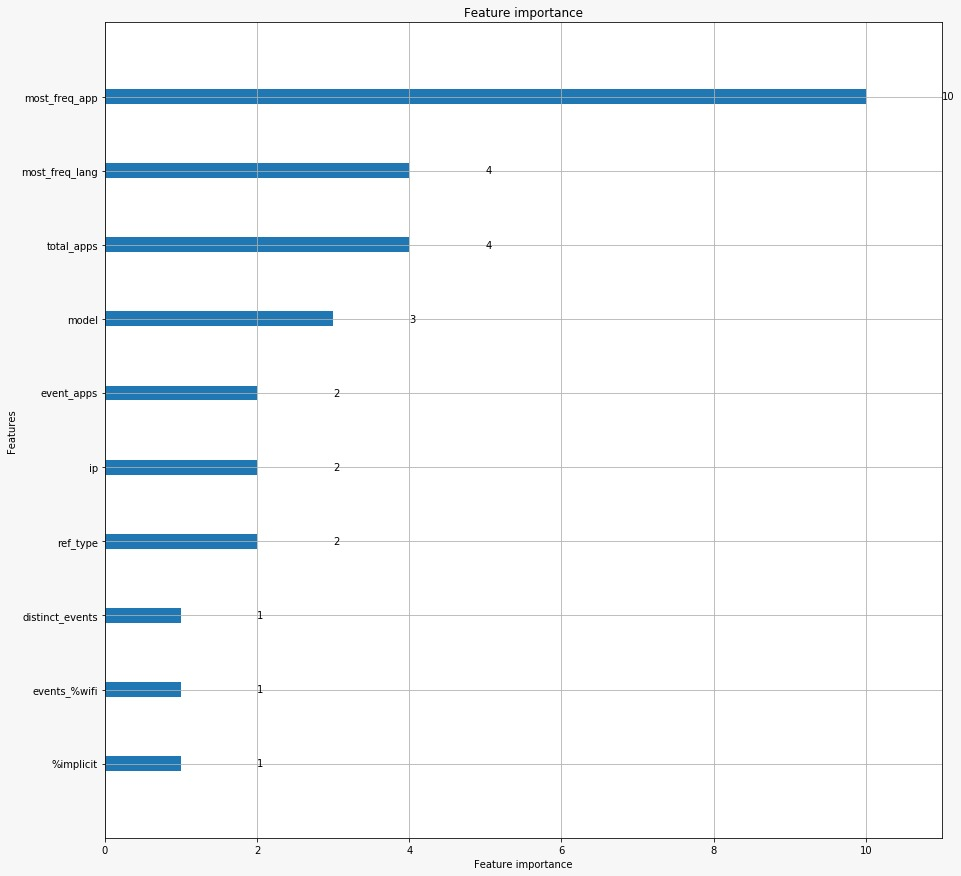
\includegraphics[width=250pt]{lgbmsc.jpeg}}
    \caption{Feature importance para LGBM sobre $Sc$}
\end{figure}

\newpage
\section{Prueba de algoritmo sencillo}
El siguiente paso fue dividir las ventanas, entrenar un algoritmo fácil de implementar y hacer un primer submit a kaggle (la plataforma en la que estaba la competencia) para verificar que se estaba siguiendo un buen camino.

Una vez divididas las siete ventanas del dataframe original, procedimos a calcular el $St$ y $Sc$ reales para cada dispositivo, para cada ventana, para poder entrenar a los algoritmos y validar. 
En el archivo \textit{auctions.csv} en cada ventana nos quedamos con las filas en las que aparecía por primera vez cada uno de los dispositivos, y le agregamos la columna $St\_real$.

En el archivo \textit{installs.csv} en cada ventana también nos quedamos con las filas en las que aparecía por primera vez cada uno de los dispositivos, y le agregamos la columna $Sc\_real$.

Luego, en ambos archivos seguimos un procedimiento similar: Para cada ventana entrenamos con XGBoost, y validamos con los siguientes tres días. Los parámetros usados fueron similares en todas la ventanas: 
(alpha=10, base\_score=0.5, booster='gbtree', colsample\_bylevel=1, colsample\_bynode=1, colsample\_bytree=0.3, gamma=0, importance\_type='gain', learning\_rate=0.8, max\_delta\_step=0, \\max\_depth=5, min\_child\_weight=1, missing=None, n\_estimators=10, n\_jobs=1, nthread=None, objective='reg:linear', random\_state=0, reg\_alpha=0, reg\_lambda=1, scale\_pos\_weight=1, seed=None, silent=None, subsample=1, verbosity=1), ya que la idea no era la busqueda de parámetros, sino simplemente probar el avance hasta el momento.

Los resultados obtenidos dieron un error cuadrático medio de entre 72000 y 80000 para St, y 50000 y 70000 para Sc

Por último se cargó el archivo target\_competencia en un dataframe, se le agregó toda la información necesaria a los dispositivos para los que se pedía predecir (mediante un join con el dataframe de auctions o installs según se quisiera el $St$ y $Sc$), y se usó el algoritmo entrenado con la ventana que mejor resultados había dado en el proceso anterior para predecir sobre esos dispostivos.

Al finalizar se hizo el primer submit a Kaggle obteniendo un error de 86368.

\newpage
\section{Prueba de algoritmos}
El siguiente paso fue usar los archivos como quedaron luego del pre-procesamiento y probar algoritmos para comparar sus resultados. La métrica usada para comparar los distintos algoritmos fue el error cuadrático medio (MSE). Cuando se hable de 'presición' en los siguientes capítulos nos referiremos al MSE.

En este paso tambíen aprovechamos para probar hiperparámetros y parámetros de los algoritmos, para ver cómo afectaban a los algoritmos.

Los algoritmos utilizados fueron XGBoost, AdaBoost, KNN, Random Forest, bagging y blending.

Tanto los algoritmos como los parámetros e hiperparámetros que se probaron pueden encontrarse en el repositorio de GitHub.

\subsection{XGBoost}
Es un algoritmo de boosting que construye la predicción a partir de la suma de resultados de varios árboles

Fue el primer algoritmo que utilizamos debido a lo sencillo de implementar usando librerías de Python, la cantidad de hiperparámetros y parámetros a setear y las buenas críticas que tiene.

Se obtuvieron buenos resultados que mejoraron un poco, aunque no mucho, modificando parámetros, tanto para $St$ como para $Sc$.

Los resultados obtenidos dieron un error cuadrático medio de entre 72000 y 80000 para St, y 50000 y 70000 para Sc (muy similares a los de la primera vez que lo probamos sin modificar hiperparámetros). Una gran ventaja de este algoritmo es la velocidad con la que entrena y predice, aún con una gran cantidad de datos

\subsection{Random Forest}
Es un algoritmo que aplica Bagging a árboles de decisión usando solo algunos atributos en cada árbol, lo que ayuda a evitar el overfitting, ya que ningún árbol tiene la totalidad de los datos para entrenar.

Con este algoritmo, y probando distintos hiperparámetros logramos para $St$ un error de entre 73000 y 80000, y para $Sc$ aproximadamente de 65000. A grandes rasgos no mejora mucho la precisión de XGBoost, aunque sí resultó de utilidad al combinarlo con otros algoritmos.

\subsection{KNN}
KNN es un algoritmo que se basa en encontrar, para un determinado punto, sus k vecinos más cercanos. Para determinar el k ideal se fue probando con distintos valores, empezando por el default, que es 5, hasta que se llegó a un k de 101 para $St$ y de 51 para $Sc$. Se emplearon estos valores ya que para valores más altos el algoritmo consumía mucho más tiempo y la ganancia en precisión no era suficiente como para justificar tal aumento.
Uno de los principales parametros a setear es la métrica a utilizar. Se entrenó al algoritmo con distintas métricas para poder elegir la mejor. Entre ellas la distancia Minkowsky con p= 1 (distancia Manhattan) y p = 2 (distancia Euclideana). La que mejor resultados entregó fue p = 2.

El error para este algoritmo fue de entre 73000 y 110000 para $St$ y de entre 66000 y 70000 para $Sc$.

Como se ve, la precisión de este algoritmo, sumado a su lentitud, hacen que no sea conveniente utilizarlo en solitario, pero si se lo utilizó en los ensambles.

\subsection{Bagging}
Otro de los algoritmos que se utilizó fue un \texttt{BaggingRegressor}, empleando dos tipos distintos de predictores de base: \texttt{KNeighborsRegressor} (KNN) y \texttt{DecisionTreeRegressor}. El trabajo de ajuste de hiperparámetros resultó largo e ineficiente, puesto que el algoritmo tarda un buen tiempo en entrenar los modelos, por lo que para determinar \texttt{max\_}\texttt{samples} y \texttt{max\_}\texttt{features} se recurrió más a la prueba y error manual. El error obtenido para las ventanas fue del rango de 66000 a 70000 para $Sc$. Se utilizó sin embargo como parte de los ensambles realizados.

\subsection{AdaBoost}
Este algoritmo de boosting fue utilizado para ambos sets, con resultados similares a los anteriores. Para $St$ se obtuvieron errores del orden de los 75000 y para $Sc$ estos se encontraban entre 64000 y 68000. Como en el caso de bagging y Knn, este algoritmo fue utilizado mayormente en ensambles, ya sea medainte averaging, blending o stacking.

\subsection{Redes neuronales}
En el caso de las redes neuronales lo que se utilizó fue lo que se conoce como \textit{Multi-Level Perceptron}, en su versión regresor. El ajuste de hiperparámetros para este resultó también largo y se debió hacer mayormente de forma manual, cambiando la función de activación hasta quedarse con una sigmoide, y modificando el \texttt{learning\_}\texttt{rate}, la cantidad de neuronas y el máximo número de iteraciones. La desventaja de este algoritmo es su extrema lentitud, que viene acompañada por una precisión considerablemente más baja que los demás algoritmos probados. Es por esto que sólo se lo utilizó como parte de ensambles y para realizar predicciones sobre $Sc$ únicamente.

Los errores para las ventanas rondaban los 85000.

\subsection{LGBM}
Se probó tambien con otro algoritmo, LightGBM, que es un algoritmo de boosting que implementa árboles de decisión. Entre las ventajas de este se encuentran su velocidad y eficiencia, ya que entrena y predice de una manera muy rápida. Sin embargo, es un algoritmo algo complejo que tiene muchos hiperparámetros, por lo que probablemente no hayamos encontrado los óptimos aún luego de realizar varias pruebas. 

Los resultados obtenidos no distaron mucho de los obtenidos con los demás algoritmos, entre 65000 y 68000.
Fue utilizado también para los ensambles.

\subsection{Ensambles}
Luego de probar los algoritmos se procedió a hacer ensambles, es decir, combinar varios algoritmos o usar las predicciones de uno o más para entrenar a algún otro algoritmo.

Esto lo hicimos entrenando los algoritmos que quisieramos usar, buscando hiperparámetros y parámetros, y buscando la mejor ventana, y poniendo las predicciones de esos algoritmos como columnas para entrenar a un nuevo algoritmo o usando el promedio de las predicciones de cada algoritmo.
En la mayoría de los casos, el algoritmo final usado para ensamblar fue XGboost.

Algunos ensambles que se probaron fueron:
\begin{itemize}
    \item Usar las predicciones de KNN para entrenar XGBoost
    \item Usar las predicciones de Random Forest y KNN para entrenar a XGBoost
    \item Usar el promedio de las predicciones de KNN, Random Forest, Bagging y XGBoost, AdaBoost
    \item Usar el promedio de las predicciones de KNN, Random Forest, Bagging, XGBoost, AdaBoost y Redes Neuronales
    \item Blending.
\end{itemize}

Los ensambles funcionaron distinto para predecir a $St$ y a $Sc$.
Los dos primeros funcionaron mejor para predecir a $St$, mientras que los dos útlimos dieron mejores resultados para predecir a $Sc$.

Para redes neuronales se usó MLP (Multi level perceptron) pero no mejoró el resultado que tenía el ensamble sin usar la red neuronal.

Lo que mejores resultados logró, y que fue lo que se uso en el mejor submit del grupo a la competencia de Kaggle hasta el momento fue:
\begin{itemize}
    \item Para $St$: Usar las predicciones de Random Forest y KNN como columnas para entrenar a XGBoost 
    \item Para $Sc$: Usar el promedio de las predicciones de los algoritmos LGBM, Random Forest, Bagging, XGBoost y AdaBoost.
\end{itemize}

Un punto importante a tener en cuenta para la prediccion de $St$ es que en un principio se buscó usar las predicciones de Random Forest y KNN como columnas para entrenar a XGBoost, lo que no generó muy buenos resultados. 
Sin embargo, decidimos probar algo un poco azaroso, que fue intercambiar dos columnas: La columna con el St real (el que se usa para entrenar) y la columna con la predicción de Random Forest. Por lo que se terminó con el $St$ real como una de las columnas para entrenar, y la predicción de Random Forest como el $St$ real.
Como era de esperarse, en las ventanas que usamos overfitteaba (se obtuvo un error cercano a 9000) pero probamos subirlo a Kaggle de todas formas y fue el que mejor resultados nos dio.

\subsubsection{Blending}
Se utilizó también la técnica de blending, para la cual se siguieron los pasos que figuran en el apunte de la materia, pero sin aplicar el \textit{Super-blender}. Para ello, se procedió para cada ventana a separar el set de entrenamiento en dos y a entrenar los algoritmos de XGBoost, Random Forests, Bagging y LGBM con una de las partes. A continuación se realizaron predicciones sobre la segunda parte y se las agregaron como features al mismo, para así entrenar a AdaBoost, con el que se realizó la predicción final.

El error obtenido con esta técnica en los submits finales fue del orden de 74000, lo cual resultó muy bueno.

Cabe destacar que si bien se obtuvieron buenos resultados con este método, no fue el que mejor rindió, lo cual contradijo las expectativas. 

\section{Conclusiones}
Como primer conclusión podemos obtener los algoritmos que mejor anduvieron. En general los mejores resultados se obtuvieron con Averaging (usando el promedio de los algoritmos implementados) tanto para $St$ como para $Sc$. La única excepción a esto fue el intercambio de columnas mencionado anteriormente para $St$.

Algo importante de notar es lo mucho que pueden variar los mismos algoritmos frente al cambio en sus parámetros y que hay algoritmos que parecen mas estables que otros. Por ejemplo, variando parámetros en XGBoost en $St$, el valor para el MSE no cambia demasiado (quizá se movia entre 70000 y 80000); mientras que Random Forest, para distintos hiperparámetros logró un error minimo cercano a 70000 y un error cercano a 110000.
Sin embargo, todos los algoritmos lograron errores mínimos muy parecidos al aplicarse por separado. Los mayores cambios se ven al hacer ensambles.

También podemos destacar que los errores podían variar considerablemente entrenando con una ventana o con otra usando el mismo algoritmo. Esto parecería indicar que los datos no son uniformes o que algunos días tienen algunos valores para $St$ o $Sc$ muy altos, lo que generaría un efecto de cisne negro.

\end{document}



